%%%%%%
%
% $Autor: Srikanth Nanda $
% $Datum: 2026-08-13 11:15:45Z $
% $Pfad: githubtemplate/Template/Presentations/Template/slides/rename.tex $
% $Version: 4620 $
%
%
% !TeX encoding = utf8
% !TeX root = Rename
%
%%%%%%

\Mysection{Introduction}
\STANDARD{Introduction}
{
\begin{figure}
	\centering
	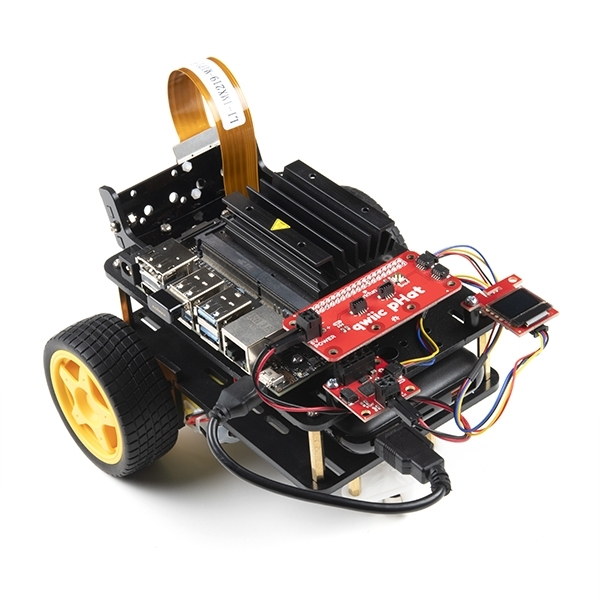
\includegraphics[width=0.5\linewidth]{images/SparkFunJetBotAIKitBack}
	\caption{Localization in a Mobile Robot}
	\label{fig:sparkfunjetbotaikitback}
\end{figure}
	\begin{itemize}
		\item Localization lets a robot estimate its \textbf{position and orientation} inside an environment
		\item Outdoor systems rely on \textbf{GPS}; indoors the signal is attenuated, reflected (multipath) and interfered with, so satellite positioning is not usable.
		\item Indoor alternatives: RF-based (Wi-Fi, Bluetooth), ultra-wideband, inertial measurement, and \textbf{vision-based} techniques.
		\item Vision-based localization estimates pose directly from image data; \textbf{monocular SLAM} additionally builds a map of the environment while tracking motion.
	\end{itemize}
	\vspace{0.3em}
%	\footnotesize Zhou, Gu \& Lu (2019); Zamir \& Shah (2010); Mur-Artal, Montiel \& Tard\'os (2015)
}
%\STANDARD{Objectives of the Thesis}
%{
%	\begin{itemize}
%		\item Develop a \textbf{vision-based indoor localization system} for a mobile robot within the \textbf{ROS} framework.
%		\item Use a \textbf{single monocular camera} as the only exteroceptive sensor for both localization and obstacle perception.
%		\item Run the complete pipeline \textbf{onboard} a resource-constrained embedded platform -- no offboard workstation for perception or control.
%		\item Complement geometric SLAM with a \textbf{learned collision-avoidance module} that closes the obstacle-perception gap pure geometry leaves open.
%		\item Validate the approach experimentally and document the practical limits: \textbf{scale ambiguity}, \textbf{temporal drift}, and \textbf{illumination sensitivity}.
%	\end{itemize}
%}
\Mysection{Problem Description} 
\STANDARD{Problem Description}
{
	
	\begin{itemize}
		\item \textbf{Task:} Indoor localization on a mobile robot.
		\item Identify the mobile robot hardware and establish indoor localizaition.
		\item Motion must therefore be recovered by \textbf{precise feature matching and tracking} across consecutive frames.
%		\item \textbf{Task:} Indoor localization on a Sparkfun JetBot mobile robot using monocular SLAM with a Leopard Imaging IMX219 camera and a 4GB 128-core NVIDIA Jetson Nano.
%		\item A monocular camera which \textbf{cannot measure absolute scale}.
%		\item Motion must therefore be recovered by \textbf{precise feature matching and tracking} across consecutive frames.
%		\item Indoor operating constraints acting on the visual pipeline:
%		\begin{itemize}
%			\item varying illumination levels,
%			\item surfaces with low texture content,
%			\item static and dynamic occlusions.
%		\end{itemize}
%		\item Pose estimation \emph{and} map generation must succeed under these conditions using only camera data and the onboard Jetson Nano.
	\end{itemize}
}

\Mysection{Challanges}
\STANDARD{Challanges}
{
	\begin{enumerate} 
		\item Geometric and perceptual challenges
	\begin{itemize}
		\item Absence of depth information $\Rightarrow$ \textbf{scale ambiguity}; absolute distances cannot be estimated from monocular views.
		\item Feature-based methods depend on \textbf{distinguishable texture}, which is not present in all indoor scenes (plain walls, reflective floors).
		\item \textbf{Temporal drift} accumulates over long trajectories without loop closure.
	\end{itemize}
		\vspace{0.4em}
	\item Environmental challenges
	\begin{itemize}
		\item Illumination changes, dynamic objects, and occlusions degrade tracking.
		\item Indoor environments introduce significant uncertainty affecting localization accuracy.
	\end{itemize}
\end{enumerate}
%	\footnotesize Mur-Artal \& Tard\'os (2017); Yassin et al. (2017)
}
\STANDARD{Challanges -- Embedded Platform}
{
	\begin{itemize}
		\item \textbf{Compute budget:} the Jetson Nano's shared 4\,GB memory and modest GPU limit the algorithmic complexity that can run in real time -- heavier stereo or LiDAR pipelines are infeasible.
		\item \textbf{Real-time safety:} obstacle reaction must happen within the control loop period, so a heavy semantic-segmentation or object-detection network is not an option.
		\item \textbf{Power:} battery-powered operation makes latency and energy per inference first-class design criteria.
		\item \textbf{Legacy software ecosystem:} JetPack 4.3 pins Ubuntu 18.04 / ROS Melodic and rosbuild-era tooling, which turned out to be the dominant practical obstacle during integration.
		\item \textbf{Dual use of one sensor:} the same camera stream must simultaneously feed the SLAM front-end and the collision classifier.
	\end{itemize}
}

\Mysection{Domain Hardware}
\STANDARD{Hardware Platform}
{		\begin{center}
		\resizebox{\textwidth}{!}{%
			\begin{tikzpicture}[node distance=3mm and 10mm]
				\node[sensor] (cam) {IMX219 CSI camera\\8MP, 20--30 fps};
				\node[hw, fill=blue!12, right=of cam, minimum width=3.0cm, minimum height=0.9cm] (nano)
				{Jetson Nano A02\\\tiny Cortex-A57 @1.43GHz, 128-core GPU, 4GB LPDDR4};
				\node[hw, fill=yellow!15, right=of nano] (batt) {Eunicell battery\\10000\,mAh};
				\node[hw, above right=8mm and -2mm of nano] (oled) {Micro OLED};
				\node[hw, below right=8mm and -2mm of nano] (qwiic) {Qwiic pHAT v2.0};
				\node[hw, below=of qwiic] (motor) {Qwiic motor driver};
				\node[hw, below=of motor] (motors) {DC motors\\(differential drive)};
				
				\draw[arr] (cam) -- node[above,font=\tiny] {CSI (single)} (nano);
				\draw[arr] (nano) -- node[above,font=\tiny] {5V} (batt);
				\draw[arr] (nano) |- node[left,font=\tiny,pos=0.75] {I2C/Qwiic} (qwiic);
				\draw[arr] (nano) |- (oled);
				\draw[arr] (qwiic) -- (motor);
				\draw[arr] (motor) -- node[left,font=\tiny] {PWM} (motors);
				\draw[arr] (batt) |- (motor.east);
				
				%				\node[draw=black!40, dashed, rounded corners, fit=(cam)(nano)(batt)(oled)(qwiic)(motor)(motors),
				%				inner sep=5mm, label={[font=\tiny]above:SparkFun JetBot v2.1}] {};
		\end{tikzpicture}}
	\end{center}
}
\STANDARD{Hardware Description}{
	\begin{itemize}
		\item \textbf{SparkFun JetBot v2.1} -- differential-drive chassis,Sparkfun Qwiic pHAT v2.0, Qwiic motor driver, micro OLED, Eunicell 10000\,mAh battery pack.
		\item \textbf{NVIDIA Jetson Nano Developer Kit A02}
		\begin{itemize}
			\item quad-core ARM Cortex-A57 @ 1.43\,GHz,
			\item 128-core Maxwell GPU, $\approx$472\,GFLOPS,
			\item 4\,GB 64-bit LPDDR4, 25.6\,GB/s bandwidth,
			\item 5\,W / 10\,W power modes at 5\,V.
		\end{itemize}
		\item \textbf{Leopard Imaging IMX219} 8\,MP H-136 CSI camera, front-mounted, 20--30\,fps.
		\item \textbf{Decisive constraint:} the A02 carrier exposes a \textbf{single usable CSI interface}  monocular vSLAM as the main geometrically grounded option.
		\item \textbf{Software baseline:} JetPack 4.3, Ubuntu 18.04, ROS Melodic.
	\end{itemize}
}
\Mysection{Proposed Solution}
\STANDARD{Proposed Solution}
{
	\begin{enumerate}
		\item Addressing scale ambiguity and texture dependence
		\begin{itemize}
		\item \textbf{Multi-view geometry and bundle adjustment} -- depth inferred by triangulating feature correspondences across multiple frames.
		\item \textbf{Loop closure} corrects accumulated drift and restores global map consistency.
		\item \textbf{ORB descriptors} give invariance to rotation, scale and illumination, improving matching in low-texture scenes.
	\end{itemize}

	\item Addressing environmental and computational limits
	\begin{itemize}
		\item \textbf{Place recognition and relocalization} to recover from tracking loss.
		\item \textbf{Outlier rejection} (RANSAC, robust loss) and temporal smoothing against dynamic elements.
		\item \textbf{Keyframe-based SLAM with local map optimization} to keep real-time performance on the Nano.
%		\item A \textbf{lightweight CNN} classifies frames as \emph{free} / \emph{blocked}, covering the obstacle-perception gap.
	\end{itemize}
\end{enumerate}
}
\STANDARD{Flowchart System Architecture}
{
	\begin{center}
		\resizebox{\textwidth}{!}{%
			\begin{tikzpicture}[node distance=6mm and 10mm]
				\node[sensor] (cam) {Monocular\\camera IMX219};
				\node[slam, above right=6mm and 10mm of cam] (orb) {ORB features};
				\node[cnn,  below right=6mm and 10mm of cam] (pre) {Preprocess\\$224\times224$};
				\node[slam, right=of orb] (pose) {Pose $+$ sparse\\map points};
				\node[cnn,  right=of pre] (onnx) {ONNX inference\\\texttt{collision\_node.py}};
				\node[block, right=14mm of $(pose)!0.5!(onnx)$] (dec) {\texttt{decision\_node.py}\\fuse pose $+$ risk};
				\node[hw, right=of dec] (cmd) {\texttt{cmd\_vel}};
				\node[hw, above=8mm of pose] (occ) {\texttt{occupancy\_grid\_node.py}};
				\node[hw, right=of occ] (map) {\texttt{map\_persistence\_node.py}};
				\node[hw, below=8mm of onnx] (tel) {\texttt{telemetry\_logger\_node.py}};
				
				\draw[arr] (cam) |- (orb);
				\draw[arr] (cam) |- (pre);
				\draw[arr] (orb) -- (pose);
				\draw[arr] (pre) -- (onnx);
				\draw[arr] (pose.east) -| (dec.north);
				\draw[arr] (onnx.east) -| (dec.south);
				\draw[arr] (dec) -- (cmd);
				\draw[arr] (pose) -- (occ);
				\draw[arr] (occ) -- (map);
				\draw[darr] (onnx) -- (tel);
				\draw[darr] (dec) |- (tel);
		\end{tikzpicture}}
	\end{center}
}
\STANDARD{System Architecture}
{
	\begin{itemize}
		\item Single camera stream is \textbf{shared} by two parallel branches:
		\begin{itemize}
			\item \textbf{vSLAM branch} -- ORB features $\rightarrow$ pose $+$ sparse map points,
			\item \textbf{CNN branch} -- free / blocked classification $\rightarrow$ collision probability.
		\end{itemize}
		\item Modular \textbf{ROS nodes}, each with explicit topics and parameters:
		\begin{itemize}
			\item \texttt{collision\_node.py} -- ONNX inference, publishes collision probability,
			\item \texttt{decision\_node.py} -- fuses pose $+$ risk, publishes \texttt{cmd\_vel},
			\item \texttt{occupancy\_grid\_node.py} -- grid from pose and map points,
			\item \texttt{map\_persistence\_node.py} -- save / reload point-cloud snapshots,
			\item \texttt{telemetry\_logger\_node.py} -- CSV logging at 1\,Hz.
		\end{itemize}
		\item \texttt{run\_jetbot\_all.sh} is a configurable orchestration layer with feature toggles (encoder odometry, telemetry, map persistence, CNN collision, camera publishing).
	\end{itemize}
}

\STANDARD{Flowchart of Pipeline}
{
		\begin{center}
		\resizebox{\textwidth}{!}{%
			\begin{tikzpicture}[node distance=6mm and 6mm]
				\node[block] (app) {1. Application:\\JetBot v2.1};
				\node[block, right=of app] (acq) {2. Data acquisition:\\camera 20--30 fps};
				\node[slam, above right=4mm and 6mm of acq] (slamb) {vSLAM: ORB $\rightarrow$\\pose $\rightarrow$ map};
				\node[cnn,  below right=4mm and 6mm of acq] (cnnb)  {CNN: frame $\rightarrow$\\$p(\text{blocked})$};
				\node[block, right=14mm of $(slamb)!0.5!(cnnb)$] (out) {4. Outlier handling:\\RANSAC / smoothing};
				\node[block, right=of out] (mon) {5. Monitoring:\\$N_{\mathrm{tracks}}(t)$, $\max_k p$};
				\node[decision, right=of mon] (anom) {Anomaly?};
				\node[block, above=8mm of anom] (resp) {6. Slow / stop /\\retrain / reinit};
				\node[block, right=of anom] (ctrl) {7. Motion control:\\pose $+$ avoidance $\rightarrow$ \texttt{cmd\_vel}};
				
				\draw[arr] (app) -- (acq);
				\draw[arr] (acq) |- (slamb);
				\draw[arr] (acq) |- (cnnb);
				\draw[arr] (slamb.east) -| (out.north);
				\draw[arr] (cnnb.east) -| (out.south);
				\draw[arr] (out) -- (mon);
				\draw[arr] (mon) -- (anom);
				\draw[arr] (anom) -- node[right,font=\tiny] {yes} (resp);
				\draw[arr] (resp) -| node[above,font=\tiny,pos=0.3] {retry} (acq.north);
				\draw[arr] (anom) -- node[above,font=\tiny] {no} (ctrl);
		\end{tikzpicture}}
	\end{center}
}
\STANDARD{Hybrid Pipeline}{
	\begin{enumerate}
		\item \textbf{Application} -- indoor robot navigation (JetBot v2.1).
		\item \textbf{Data acquisition} -- front-facing monocular camera at 20--30\,fps.
		\item \textbf{Parallel perception}
		\begin{itemize}
			\item vSLAM: ORB features $\rightarrow$ pose $\rightarrow$ sparse map,
			\item CNN: preprocessed frame $\rightarrow$ $p(\text{blocked})$.
		\end{itemize}
		\item \textbf{Outlier handling} -- RANSAC / robust loss on the geometric side, temporal smoothing and safety rules on the learned side.
		\item \textbf{Monitoring} -- number of tracked features $N_{\mathrm{tracks}}(t)$ and maximum class probability $\max_k p(y=k\,|\,I_t)$.
		\item \textbf{Anomaly response} -- reduce speed, safe stop, retrain; persistent anomalies trigger reinitialization and new data collection.
		\item \textbf{Motion control} -- pose $+$ avoidance decision $\rightarrow$ bounded wheel command.
	\end{enumerate}

}


\Mysection{Methodology}
\STANDARD{Methodology}
{
	\begin{itemize}
		\item No single framework covers the work; \textbf{three complementary layers} are combined:
		\begin{itemize}
			\item \textbf{CRISP-DM} structures the project at engineering level,
			\item the \textbf{KDD process} governs how raw sensor data becomes usable knowledge,
			\item a standard \textbf{ML pipeline} covers the concrete CNN implementation.
		\end{itemize}
		\item \textbf{Justification}
		\begin{itemize}
			\item the single CSI interface forces monocular vSLAM,
			\item real-time safety forces a lightweight learned classifier,
			\item the ROS design allows every node to be validated independently before integrated testing.
		\end{itemize}
		\item An ML system is more than its algorithm: it also comprises the data pipeline, the evaluation protocol, and the deployment and monitoring infrastructure.
	\end{itemize}
}
\STANDARD{CRISP-DM}
{
	\begin{center}
		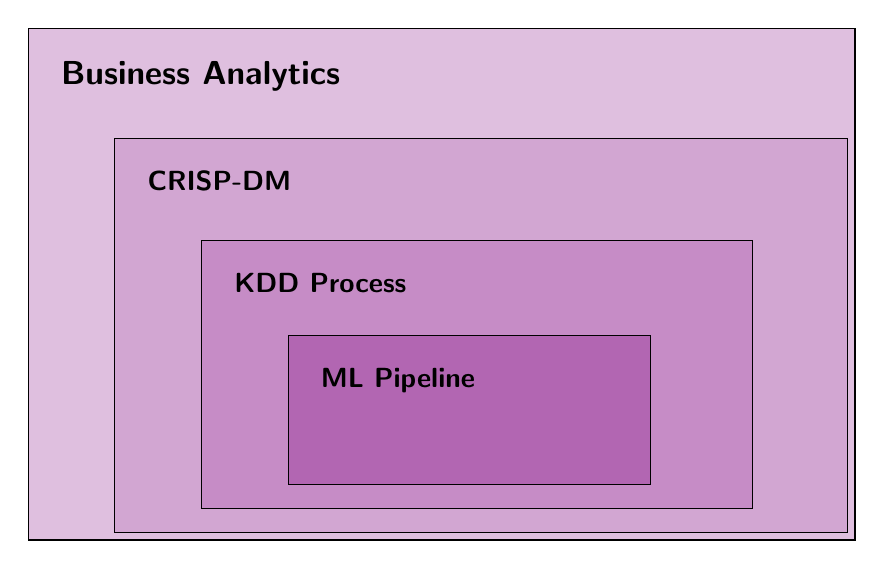
\begin{tikzpicture}[font=\sffamily]
			\node[draw, fill=violet!25, minimum width=10.5cm, minimum height=6.5cm, anchor=north west, align=left, font=\sffamily\bfseries\large] (ba) at (0,0) {};
			\node[anchor=north west, xshift=3mm, yshift=-3mm, font=\sffamily\bfseries\large] at (ba.north west) {Business Analytics};
			
			\node[draw, fill=violet!35, minimum width=9.3cm, minimum height=5.0cm, anchor=north west, font=\sffamily\bfseries] at (1.1,-1.4) (crisp) {};
			\node[anchor=north west, xshift=3mm, yshift=-3mm, font=\sffamily\bfseries] at (crisp.north west) {CRISP-DM};
			
			\node[draw, fill=violet!45, minimum width=7.0cm, minimum height=3.4cm, anchor=north west, font=\sffamily\bfseries] at (2.2,-2.7) (kdd) {};
			\node[anchor=north west, xshift=3mm, yshift=-3mm, font=\sffamily\bfseries] at (kdd.north west) {KDD Process};
			
			\node[draw, fill=violet!60, minimum width=4.6cm, minimum height=1.9cm, anchor=north west, font=\sffamily\bfseries] at (3.3,-3.9) (ml) {};
			\node[anchor=north west, xshift=3mm, yshift=-3mm, font=\sffamily\bfseries] at (ml.north west) {ML Pipeline};
		\end{tikzpicture}
	\end{center}
	\begin{description}
		\item[Task] Navigation defined as monocular vSLAM plus CNN-based collision avoidance on embedded hardware largely forced by the single CSI camera interface.
		\item[Database] Camera stream, pose topic and collision-probability topic characterized by quantity, quality and known failure modes (illumination sensitivity, low texture, scale ambiguity).
		\item[Data Preparation] Captured frames cleaned, deduplicated and augmented.
		\item[Modeling] CNN collision classifier trained and integrated with ORB-SLAM2 pose output.
		\item[Evaluation] Classifier and system-level performance quantified against held-out data and integrated runs.
		\item[Deployment] Trained model exported to ONNX and promoted into the runtime ROS graph.
	\end{description}
	\vspace{0.2em}
%	\footnotesize The lifecycle is deliberately \emph{iterative}: error analysis in later phases sends work back to labeling and data engineering.
}
\STANDARD{KDD}
{
	\begin{itemize}
		\item \textbf{Selection} -- forward-facing navigation scenes from the JetBot camera logs: free-path motion, close obstacle approaches, reflective surfaces, low-texture regions.
		\item \textbf{Preprocessing / Cleaning} -- \texttt{cnn\_kdd\_transform.py} computes perceptual hashes to catch duplicate frames and a Laplacian-variance blur score to flag low-quality images.
		\item \textbf{Transformation} -- resize to $224\times224$, channel reordering, normalization with fixed channel mean and standard deviation.
		\item \textbf{Data Mining} -- \texttt{cnn\_train\_tf.py} trains a compact convnet from scratch with aggressive augmentation and close validation-loss monitoring.
		\item \textbf{Interpretation / Evaluation} -- outputs read as collision probabilities, checked offline and in integrated hardware trials.
	\end{itemize}
	\vspace{0.3em}

}

\Mysection{Development}
\STANDARD{Development -- Datasets}
{
	Two datasets with distinct roles, instead of a conventional DBMS:
	\vspace{0.4em}
	\textbf{Blocked / free image dataset}
	\begin{itemize}
		\item Collected directly from the JetBot's onboard monocular camera by teleoperation.
		\item \textbf{Free} -- clear, navigable path, no immediate obstacle.
		\item \textbf{Blocked} -- wall, furniture or other object within collision range.
		\item Purpose: train a lightweight CNN able to run in real time on the Nano and modulate motor commands.
	\end{itemize}
}

%\STANDARD{Development -- CNN Architecture}
%{
%	Lightweight sequential CNN trained \textbf{from scratch}, deliberately not a pretrained ResNet/VGG backbone (tens of millions of parameters would strain the Nano's shared 4\,GB memory).
%	\vspace{0.4em}
%	\begin{center}
%		\footnotesize
%		\begin{tabular}{ll}
%			\hline
%			\textbf{Parameter}              & \textbf{Value}          \\
%			\hline
%			Conv filters (block 1 / 2 / 3)  & 16 / 32 / 64            \\
%			Kernel size                     & $3\times3$              \\
%			Activation                      & ReLU                    \\
%			Pooling                         & MaxPooling2D $2\times2$ \\
%			Head                            & GlobalAvgPool / Dense 64 \\
%			Output                          & 1 neuron, sigmoid       \\
%			Optimizer                       & Adam                    \\
%			Loss                             & Binary cross-entropy    \\
%			Batch size                      & 16--32                  \\
%			Epochs                          & 20--30                  \\
%			\hline
%		\end{tabular}
%	\end{center}
%}
\STANDARD{Development -- CNN Observations}
{
	\textbf{Critical detail:} the identical preprocessing function is reused unmodified at inference time, and the ONNX manifest records input size, channel ordering and normalization so \textbf{training--serving skew} can be verified rather than assumed.
	
	Filter counts double with depth: shallow layers capture edges and texture, deeper layers task-specific patterns. Optimised lightweight CNNs on edge devices report up to \textbf{65\% lower latency} and \textbf{45\% lower energy} than uncompressed CNNs while staying above 90\% accuracy.
%	(Chatterjee et al., 2023; Zuffo et al., 2024).
}
\STANDARD{Development -- SLAM Integration}
{
	\begin{itemize}
		\item \textbf{Dependency compilation:} Pangolin, DBoW2 and OpenBLAS built from source on the Nano.
		\item \textbf{ORB-SLAM2} built successfully as a \textbf{standalone library}; repository structure intact.
		\item \textbf{ROS bridge:} catkin workspace with camera integration, containerized bring-up, network configuration.
		\item \textbf{ORB-SLAM3} configured for monocular mode (camera intrinsics, vocabulary path, sensor mode) and validated on \texttt{freiburg1\_xyz} -- tracking, local mapping and loop-closing threads visible in the Pangolin viewer.
	\end{itemize}
}
\STANDARD{Development -- Integration blockers}
{
	\textbf{Integration blockers encountered:}
	\begin{itemize}
		\item Python bindings fail with an \textbf{undefined symbol} in the Boost/OpenCV converter layer,
		\item rosbuild-based examples cannot obtain compile flags because \texttt{rospack} fails on a \texttt{python-catkin-pkg} dependency under JetPack 4.3 / ROS Melodic,
		\item the launch configuration references a non-existent \texttt{orb\_slam2\_ros} package.
	\end{itemize}
	
}
\STANDARD{Development -- Model Export}
{
	\begin{figure}[H]
		\centering
		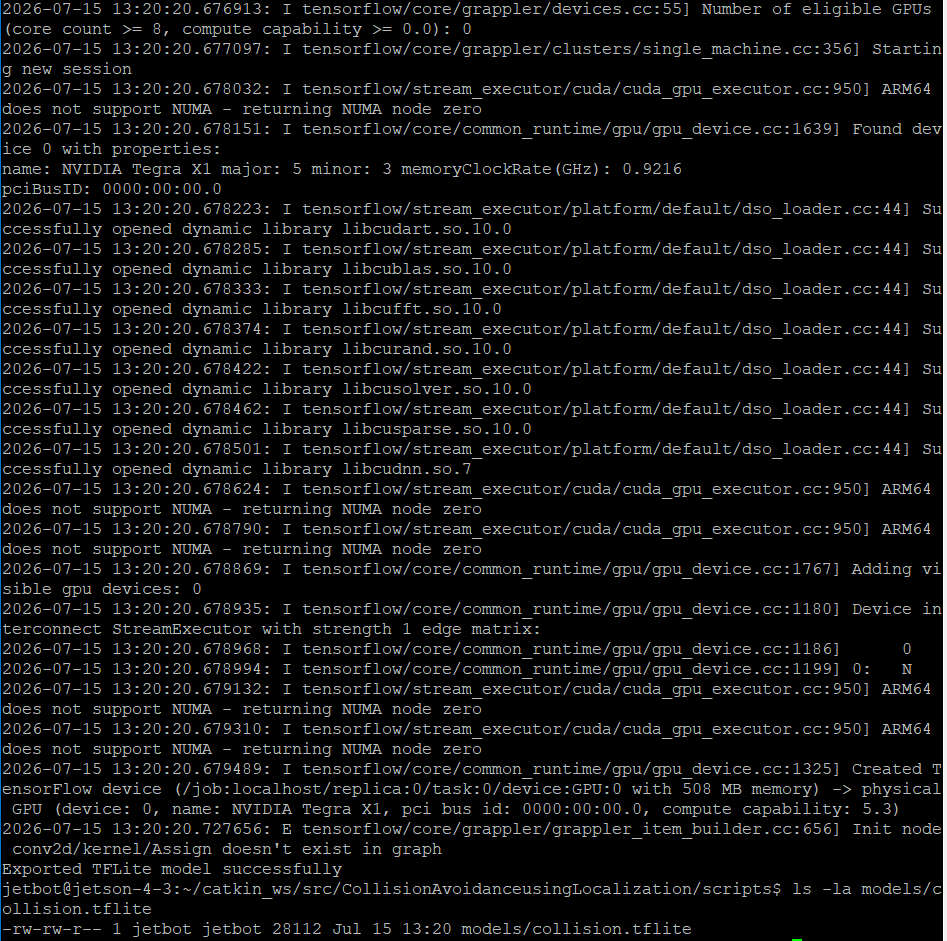
\includegraphics[width=0.5\linewidth]{images/Collision_TFLite_Model_Verification}
		\caption{Collision Tensorflow Lite Model Verification}
		\label{fig:collisiontflitemodelverification}
	\end{figure}
	\begin{itemize}
		\item \textbf{Training pipeline:} load and preprocess images, split train/validation/test, build the sequential model, compile with Adam and binary cross-entropy, train with augmentation (flips, brightness jitter).
		\item \textbf{Export chain:} frozen graph $\rightarrow$ SavedModel $\rightarrow$ TFLite $\rightarrow$ \textbf{ONNX}, with GPU initialization and TensorFlow pipeline debugging documented at each step.
		\item \textbf{Manifest:} \texttt{cnn\_dev\_to\_deploy.py} writes input tensor size, channel ordering and normalization parameters alongside the artifact.
		\item \textbf{Promotion:} \texttt{cnn\_deploy\_model.py} uses hashing and manifest verification -- a champion/challenger discipline at small-system scale; a new ONNX artifact is only promoted after its manifest verifies.
		\item \textbf{Data version control:} environment setup and dataset versioning so a retrained model follows the same validated path as the original.
	\end{itemize}
}
\Mysection{Evaluation}
\STANDARD{Evaluation}
{
Can the JetBot maintain a stable pose estimate while avoiding obstacles in real time, i.e. localize, classify risk and issue safe velocity commands without human intervention?
	\vspace{0.4em}
	\begin{itemize}
		\item \textbf{Metrics} computed by \texttt{cnn\_evaluate.py} against a labeled test set: confusion matrix, accuracy, precision, recall, F1, and \textbf{average inference latency}; results optionally written to JSON.
		\item Decision threshold default $0.60$; input $224\times224$, ImageNet-style mean/std normalization, ONNX executed through \texttt{cv2.dnn}.
%		\item Held-out evaluation only -- the test set is never touched during training or hyperparameter tuning.
		\item \textbf{Application:} corridor runs, obstacle approaches and recovery scenarios; every run records camera stream, pose, collision probability and command output for post-hoc inspection.
	\end{itemize}

}
\STANDARD{Evaluation -- Validation}
{
	Current status is \textbf{partial functional validation}, not full system validation.
%	: separate nodes exist for control, map building, persistence, telemetry and model deployment, each with explicit topics and parameters.
	\begin{enumerate}
		\item \textbf{CNN-only navigation validation} -- run the deployed ONNX model, route the decision node to the CNN collision topic, and measure whether the JetBot sustains obstacle-free reactive motion in a known corridor.
		\item \textbf{Map-collision and occupancy-grid validation} -- exercise the occupancy-grid and map-persistence nodes with recorded or simulated pose and sparse point-cloud inputs, no live SLAM required.
		\item \textbf{Split-environment validation} -- ONNX and control stack on the JetBot, ORB-SLAM2/3 trajectory and map generation in a better-supported offline environment, then compare expected SLAM-enhanced behaviour against deployable JetBot behaviour.
	\end{enumerate}
%	\footnotesize Offline evaluation is treated as a \textbf{gate}, not a final verdict -- staged rollout remains necessary.
}
\Mysection{Monitoring}
\STANDARD{Monitoring}
{
	\textbf{Idea:} model and data quality degrade \emph{quietly} once a system leaves development; ML systems fail silently because predictions keep arriving without any crash. The same telemetry used to validate lab experiments must also catch degraded camera input, stale pose estimates or abnormal collision probabilities in autonomous operation at near-zero compute overhead.
}
%\STANDARD{Monitoring Implementation}
%{
%	\begin{itemize}
%		\item \textbf{Pre-flight:} \texttt{cnn\_pipeline\_monitor.py} waits with bounded timeout for messages on pose, collision-probability, collision-risk and \texttt{cmd\_vel} topics before an experiment starts.
%		\item \textbf{Rate checks:} degraded camera stream flagged below \textbf{5\,Hz} on \texttt{camera/image\_raw}; degraded control loop below \textbf{1\,Hz} on \texttt{cmd\_vel}.
%		\item \textbf{Runtime:} \texttt{telemetry\_logger\_node.py} logs pose, odometry, \texttt{cmd\_vel}, collision probability, collision flags and battery state to CSV at 1\,Hz.
%		\item \textbf{Feedback loop:} anomalies such as, not a fixed schedule, triggering new data collection and retraining through the same KDD stages.
%		\item \textbf{Privacy \& robustness:} frames and logs stay local to the Nano; monitoring runs independently of the safety-critical decision node.
%	\end{itemize}
%}
\Mysection{Deployment}
\STANDARD{Deployment}
{
	\begin{itemize}
		\item \textbf{Pipeline:} camera data collection on the JetBot $\rightarrow$ offline training of the collision-risk classifier $\rightarrow$ copying the exported model and ROS package onto the NVIDIA Jetson Nano.
	\end{itemize}
		\begin{figure}[H]
			\centering
			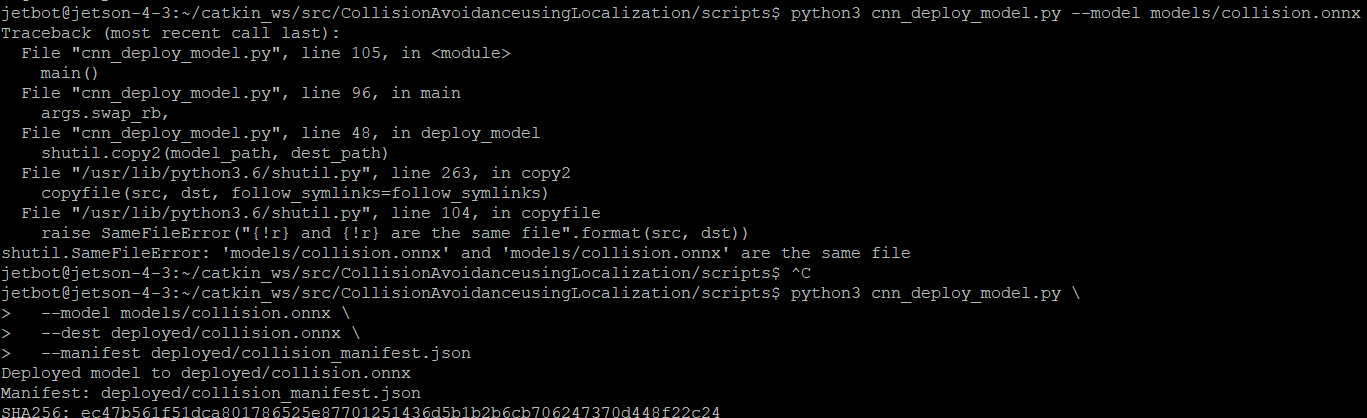
\includegraphics[width=\linewidth]{images/ONNX_Model_Deployment_Success}
			\caption{Successful Deployment of CNN Model}
			\label{fig:onnxmodeldeploymentsuccess}
		\end{figure}
}
\STANDARD{Deployment Phase 2}
{
			\begin{itemize}
		\item Pose estimator, collision inference node and motion decision node all live in \textbf{one ROS workspace}, keeping the control loop local to the robot.
		\item Reproducible versioning ensures the exact artifact validated offline is the one that runs on the robot.
		\item \texttt{run\_jetbot\_all.sh} supports copying a chosen model into \texttt{models/collision.onnx} and can route the control node either to map-based collision output or to a CNN-based collision topic.
	\end{itemize}
	\vspace{0.3em}
%	\footnotesize Huyen (2022); G\'eron (2022); Chollet (2021); Mur-Artal \& Tard\'os (2017)
}
\STANDARD{Deployment -- Orchestration}
{
	Orchestration of \texttt{run\_jetbot\_all.sh}:
	\begin{enumerate}
		\item Parse command-line arguments and set feature flags.
		\item \textbf{Checks-only mode?} $\rightarrow$ run requested pre-flight checks: \texttt{--camera-test}, \texttt{--calibrate}, \texttt{--qwiic-test}.
		\item Otherwise: deploy the CNN model if \texttt{--model-path} is given.
		\item Start the camera publisher if \texttt{--start-camera-pub}.
		\item Launch \texttt{system.launch} with all feature toggles and the selected collision topic -- camera driver, SLAM node, occupancy grid, collision node, decision controller and telemetry logger, in order and with startup delays.
		\item Optionally run \texttt{cnn\_pipeline\_monitor.py} (\texttt{--monitor}) and \texttt{cnn\_data\_collect.py} (\texttt{--collect-data}).
		\item Wait for \texttt{roslaunch}, then clean up.
	\end{enumerate}
}
\Mysection{Results}
\STANDARD{Results -- Perception and Localization}
{
	\begin{itemize}
		\item \textbf{CNN training completed:} final-epoch logs confirm convergence and a saved model checkpoint; precision, recall and accuracy computed on the validation set.
		\item \textbf{ONNX evaluation:} accuracy and average latency of the exported ONNX model compared against the original TensorFlow model verified after training.
		\item \textbf{Live test:} collision-detection model exercised on live JetBot camera input.
		\item \textbf{ORB-SLAM3 on TUM RGB-D:} successful execution on \texttt{freiburg1\_xyz}: real-time sparse 3D point cloud, keyframe trajectory and live feature tracking in Pangolin; full camera trajectory generated and saved for accuracy evaluation.
		\item \textbf{Build validation:} ORB-SLAM3 shared libraries linked with no unresolved symbols; ROS2/colcon workspace configured for publishing localization data.
	\end{itemize}
}
\STANDARD{Results -- Integration Findings}
{
	\begin{enumerate}
	\item Observations
	\begin{itemize}
		\item ORB-SLAM2 built as a standalone library; complete Python navigation stack with deployment script, telemetry logger, occupancy-grid node and reactive decision node.
		\item The decision node implements a usable reactive policy: slow-down and stop thresholds, recovery turning, optional reversing, heading stabilization.
	\end{itemize}
	\item Drawbacks
	\begin{itemize}
		\item \textbf{ROS integration} blocked -- rosbuild examples cannot obtain compile flags after \texttt{rospack} fails on \texttt{python-catkin-pkg} under JetPack 4.3 / ROS Melodic.
		
		\item Bring-up reaches launch but shuts down on the missing \texttt{orb\_slam2\_ros} package: only \texttt{/rosout} remains, i.e. \textbf{no navigation nodes active}.
	\end{itemize}
	\end{enumerate}
}
\Mysection{Conclusion}
\STANDARD{Conclusion}
{
	\begin{itemize}
		\item The work produced a \textbf{well-structured onboard navigation software stack}, but not yet a stable end-to-end deployment of monocular ORB-SLAM2 on the Jetson Nano under JetPack 4.3 / ROS Melodic.
		\item Strongest practical outcome: a \textbf{deployable ONNX-based collision-avoidance pipeline} with ROS orchestration, telemetry logging and modular support for occupancy grids and map persistence.
		\item The central limitation is not architectural design but the \textbf{fragility of the software integration boundary} between ORB-SLAM2, ROS and Python bindings on this platform.
	\end{itemize}
}
	\STANDARD{Self-critical}
	{
		\begin{itemize}
			\item Effort went into high-risk integration before a minimal working baseline was frozen; SLAM should have been an incremental extension, not an early dependency.
			\item Device-level trajectory results could not be reported for confidentiality reasons, so the \textbf{TUM RGB-D benchmark} serves as a controlled substitute, it isolates algorithmic performance but not the real corridor's lighting, texture and motion characteristics.
			\item \textbf{Open questions:} whether the JetPack 4.3 limitation is repairable at acceptable cost; how robust CNN-only navigation is across lighting and texture variation; and whether persistent map reuse can support long-term autonomy.
		\end{itemize}
	}
	\Mysection{Next Steps}
	\STANDARD{Next Steps}
	{
		
		\begin{itemize}
			\item \textbf{Minimal successful run:} refactor the launch configuration so all \texttt{orb\_slam2\_ros} references become optional flags, start the stack in CNN-only mode, and verify live topics for camera input, collision output and non-zero \texttt{cmd\_vel} in a short bench test.
			\item \textbf{Repeatable indoor trials:} run the ONNX collision pipeline on a fixed test route with CSV telemetry enabled, reporting run duration, command stability, collision events and battery state instead of only software architecture.
			\item \textbf{Platform upgrade:} flashing JetPack 4.5 is performed using BalenaEtcher in compatible SD Card.
\begin{figure}[H]
	\centering
	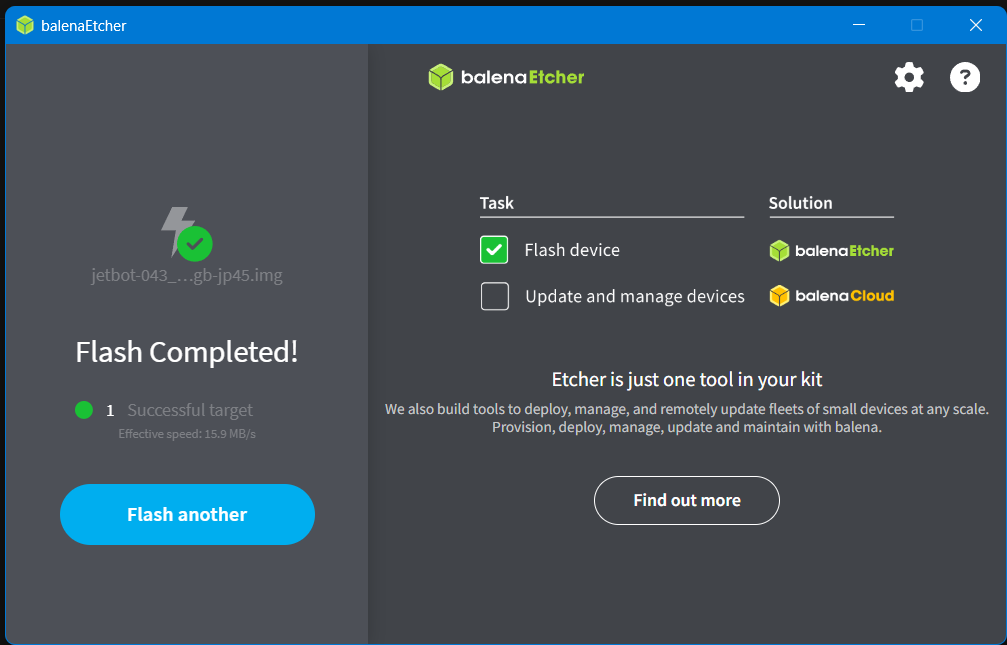
\includegraphics[width=0.7\linewidth]{images/EtcherSuccessful}
	\caption{Flashing Successful NVIDIA Jetbot - Jetpack 4.5 in SD Card}
	\label{fig:etchersuccessful}
\end{figure}
		\end{itemize}
		}
		\STANDARD{Next Steps -- Hardware Consideration}
		{
			\begin{itemize}
			\item \textbf{Reposition ORB-SLAM2} as an offline evaluation tool or future extension unless the ROS environment can be established on another platform.
			\item While keeping the work technically professional while preserving the Monocular Visual Simultaneous Localization and Mapping ambition, and highlighting the contribution: a modular mobile robot autonomy stack that shows exactly where monocular SLAM integration becomes difficult on constrained, legacy embedded software environments like NVIDIA Jetson Nano.
		\end{itemize}
	}
	
\Mysection{Delighter}
\STANDARD{Delighter -- Independent Cross-Platform Validation}
{
	\begin{itemize}
		\item While the NVIDIA JetPack~4.3 integration hit the blockers on the previous slide, the \textbf{same monocular ORB-SLAM3 pipeline} was independently built, debugged and validated end-to-end on \textbf{two different platforms outside the target hardware}: a laptop (WSL2/Ubuntu) and a smartphone camera stream.
		\item \textbf{Live tracking confirmed:} real-time keyframe tracking, local mapping and loop-closing threads visible in the Pangolin viewer.
%		\item \textbf{Map persistence confirmed:} the Atlas map was saved (\texttt{SaveAtlasToFile}) and successfully reloaded (\texttt{LoadAtlasFromFile}) for relocalization against a previously built map to verify the save/load cycle needed for any future map-based navigation step.
		\item \textbf{Why this matters:} it isolates the JetBot shortfall to the \textbf{JetPack~4.3 / ROS Melodic integration layer} (Python/Boost bindings, \texttt{rospack}/\texttt{catkin} tooling) and not to the monocular VSLAM method, the calibration approach, or the underlying understanding of the algorithm.
	\end{itemize}
}

\STANDARD{Delighter -- Engineering Behind the Validation}
{
	\textbf{Non-trivial fixes required to reach a stable, reproducible pipeline:}
	\begin{itemize}
		\item \textbf{Build isolation:} removed leftover ROS/catkin \texttt{find\_package} block from \texttt{CMakeLists.txt} to stop the linker silently merging two incompatible OpenCV versions (system 4.2 vs.\ source-built 4.4) into \texttt{libORB\_SLAM3.so}.
		\item \textbf{Linking fix:} explicitly linked GLEW against Pangolin's OpenGL calls to resolve an undefined-reference failure at build time.
%		\item \textbf{Source-code correction:} removed a leftover debug hack in \texttt{Frame::ComputeBoW()} that misreported normal keyframe/relocalization activity as false or lost track events.
		\item \textbf{Streaming robustness:} added frame-validity checks and monotonic-timestamp enforcement in the capture loop to handle corrupted MJPEG frames and clock drift over a live network stream.
		\item \textbf{Camera calibration:} performed a full checkerboard calibration (intrinsics + distortion) rather than relying on a zero-distortion placeholder, since drift and tracking loss are highly sensitive to calibration accuracy.
		\begin{figure}[H]
			\centering
			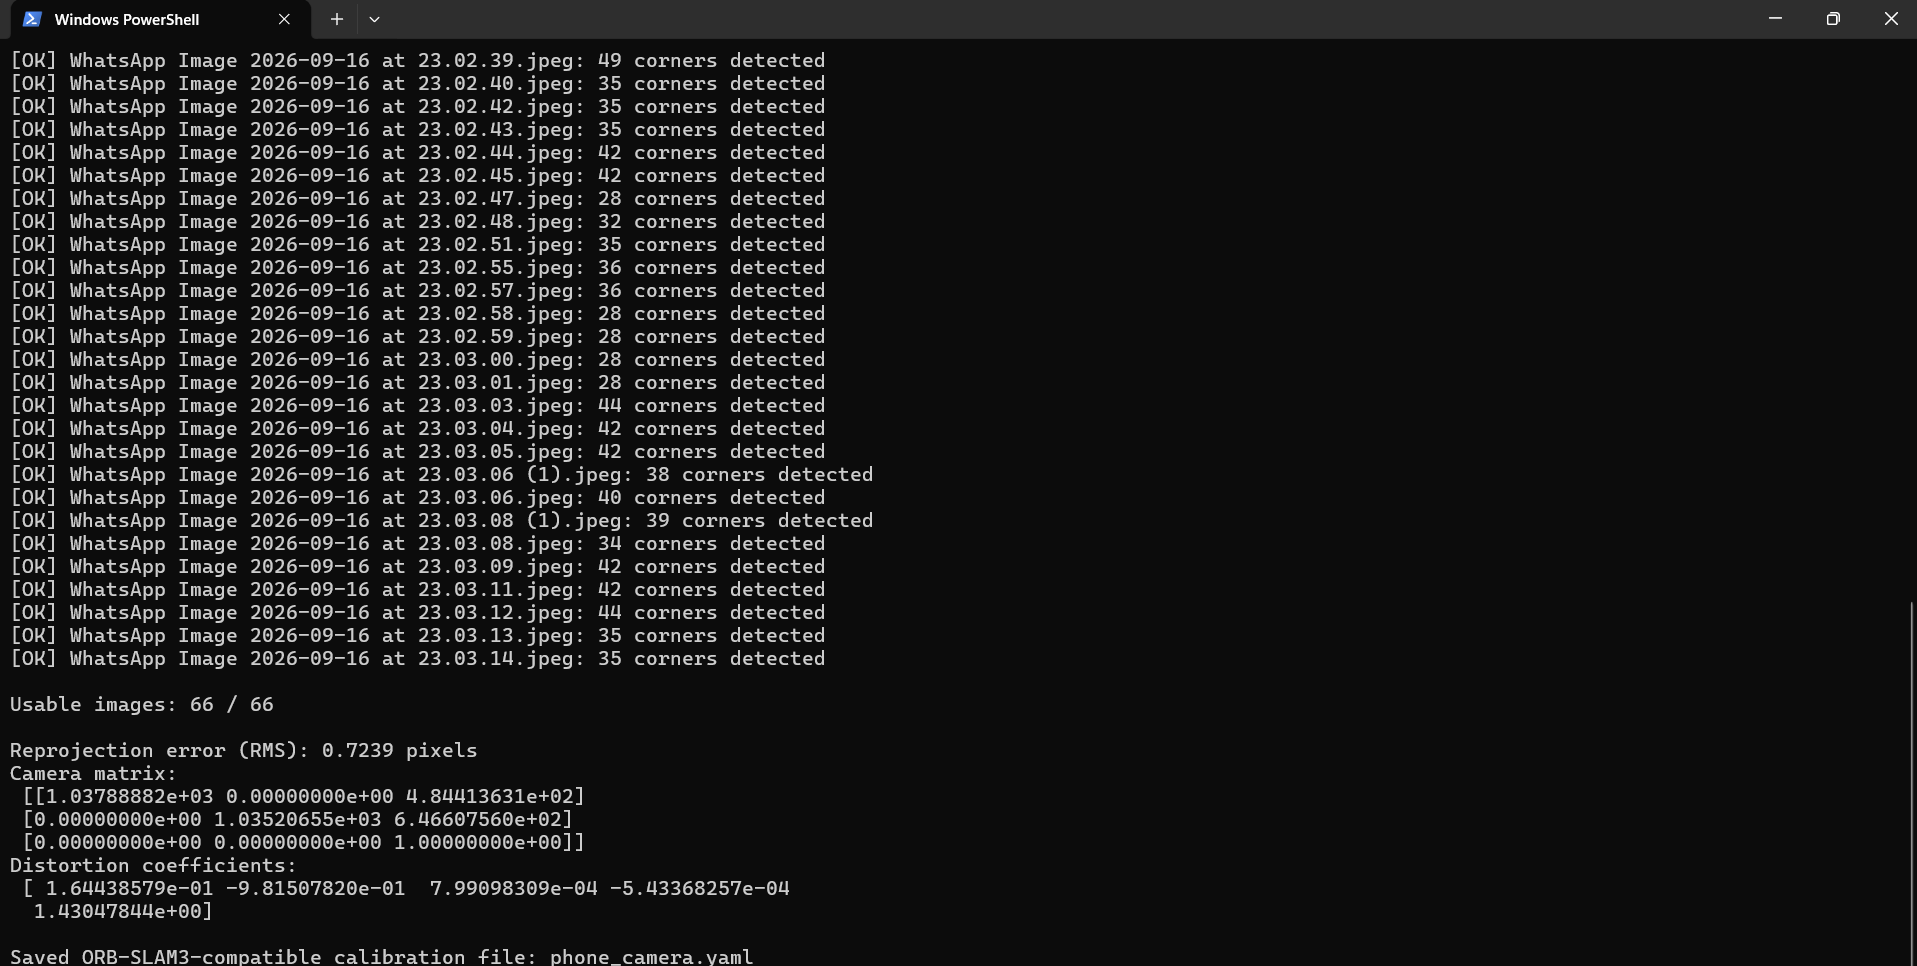
\includegraphics[width=\linewidth]{images/MobileCameraCalibration}
			\caption{Mobile Camera Calibration}
			\label{fig:mobilecameracalibration}
		\end{figure}
	\end{itemize}
}